\section*{Nmap}
\subsection*{Standard TCP Connection Scan of \texttt{compeng4dn4.mooo.com}}
A standard TCP connection scan (using -sT option) of the server \texttt{compeng4dn4.mooo.com} over the port range 50000-50009 is performed and shown in Listing~\ref{list:nmap_mooo_sT}. The scan showed that ports 50007 and 50008 were open, indicating that \href{https://nmap.org/book/man-port-scanning-basics.html}{there is an application that will accept TCP connections, UDP datagrams, or SCTP associated on these ports}. The remainder of the ports reported their states as filtered, indicating Nmap could not determine if the port is open. Nmap states that this usually occurs due to \href{https://nmap.org/book/man-port-scanning-basics.html}{packet filtering preventing Nmap's probes from reaching the port}. The known services corresponding with each port (from the \href{https://nmap.org/book/man-version-detection.html}{nmap-services} database) are also listed, with port 50000 being used for IBM Db2 and port 50002 for \href{http://openi18n.web.fc2.com/subgroups/im/IIIMF/faq/FAQ.html}{Internet/Intranet Input Method Server Framework}.

\begin{lstlisting}[caption=Nmap Standard TCP Connection Scan Over Port Range 50000-50009,label=list:nmap_mooo_sT]
nmap compeng4dn4.mooo.com -Pn -sT -p 50000-50009
Starting Nmap 7.93 ( https://nmap.org ) at 2023-02-11 22:50 Eastern Standard Time
Nmap scan report for compeng4dn4.mooo.com (99.236.34.223)
Host is up (0.030s latency).
rDNS record for 99.236.34.223: cpe382c4a5bff48-cm00fc8db8cbb0.cpe.net.cable.rogers.com

PORT      STATE    SERVICE
50000/tcp filtered ibm-db2
50001/tcp filtered unknown
50002/tcp filtered iiimsf
50003/tcp filtered unknown
50004/tcp filtered unknown
50005/tcp filtered unknown
50006/tcp filtered unknown
50007/tcp open     unknown
50008/tcp open     unknown
50009/tcp filtered unknown

Nmap done: 1 IP address (1 host up) scanned in 3.36 seconds
\end{lstlisting}


\subsection*{TCP SYN Scan of \texttt{compeng4dn4.mooo.com}}
A TCP SYN scan (using -sS option) of the server \texttt{compeng4dn4.mooo.com} over the port range 50000-50009 is performed and shown in Listing~\ref{list:nmap_mooo_sS}. The scan returns the same information, reporting the same state and services for each of the ports scanned.

\begin{lstlisting}[caption=Nmap TCP SYN Scan Over Port Range 50000-50009,label=list:nmap_mooo_sS]
nmap compeng4dn4.mooo.com -Pn -sS -p 50000-50009
Starting Nmap 7.93 ( https://nmap.org ) at 2023-02-11 22:51 Eastern Standard Time
Nmap scan report for compeng4dn4.mooo.com (99.236.34.223)
Host is up (0.032s latency).
rDNS record for 99.236.34.223: cpe382c4a5bff48-cm00fc8db8cbb0.cpe.net.cable.rogers.com

PORT      STATE    SERVICE
50000/tcp filtered ibm-db2
50001/tcp filtered unknown
50002/tcp filtered iiimsf
50003/tcp filtered unknown
50004/tcp filtered unknown
50005/tcp filtered unknown
50006/tcp filtered unknown
50007/tcp open     unknown
50008/tcp open     unknown
50009/tcp filtered unknown

Nmap done: 1 IP address (1 host up) scanned in 1.50 seconds
\end{lstlisting}

\subsection*{TCP Scans of Open Port 50007}
A standard TCP connection scan (using -sT option) and a TCP SYN scan (using -sS option) of the server \texttt{compeng4dn4.mooo.com} on the open port 50007 are performed and shown in Listing~\ref{list:nmap_50007}. For both scans, the Nmap scan reported the same information. The scans reported the same information on port 50007 as the earlier scans on the larger port range.

\begin{lstlisting}[caption=Nmap Scans on Port 50007,label=list:nmap_50007]
sudo nmap compeng4dn4.mooo.com -Pn -sT -p 50007
Starting Nmap 7.80 ( https://nmap.org ) at 2023-02-12 21:32 EST
Nmap scan report for compeng4dn4.mooo.com (99.236.34.223)
Host is up (0.031s latency).
rDNS record for 99.236.34.223: cpe382c4a5bff48-cm00fc8db8cbb0.cpe.net.cable.rogers.com

PORT      STATE SERVICE
50007/tcp open  unknown

Nmap done: 1 IP address (1 host up) scanned in 0.15 seconds

sudo nmap compeng4dn4.mooo.com -Pn -sS -p 50007
Starting Nmap 7.80 ( https://nmap.org ) at 2023-02-12 21:32 EST
Nmap scan report for compeng4dn4.mooo.com (99.236.34.223)
Host is up (0.024s latency).
rDNS record for 99.236.34.223: cpe382c4a5bff48-cm00fc8db8cbb0.cpe.net.cable.rogers.com

PORT      STATE SERVICE
50007/tcp open  unknown

Nmap done: 1 IP address (1 host up) scanned in 0.20 seconds
\end{lstlisting}

Both scans were captured with tcpdump, writing the scan to a WireShark compatible pcap file for analysis. The tcpdump packet capture command of the scans is shown in Listing~\ref{list:tcpdump_50007}. 

\begin{lstlisting}[caption=Tcpdump Packet Capture of Scans on Port 50007,label=list:tcpdump_50007]
sudo tcpdump -nnvvX -i 1 -S host compeng4dn4.mooo.com -w 50007.pcap
tcpdump: listening on eth0, link-type EN10MB (Ethernet), snapshot length 262144 bytes
7 packets captured
13 packets received by filter
0 packets dropped by kernel
\end{lstlisting}

The capture displayed in WireShark is shown below in Figure~\ref{fig:wireshark_50007}. The first four packets (1-4) are from the standard TCP connection scan on port 50007. The last three packets (5-7) are from the TCP SYN scan on port 50007.

The first four packets shows the \href{https://nmap.org/book/scan-methods-connect-scan.html#scan-methods-fig-connect-scan-open}{expected behaviour of a TCP connection scan on an open port}. The host (192.168.2.55) sends a SYN signal to the destination (port 50007 on 99.236.34.223). The destination lets the host know that the port is open by returning a SYN/ACK signal. The host then establishes the connection and sends an ACK signal. Finally, the host will kill the connection with a RST signal.

The last three packets shows the \href{https://nmap.org/book/synscan.html#scan-methods-fig-syn-scan-open}{expected behaviour of a TCP SYN scan on an open port}. The first two packets are the same as before, however the host sends a RST signal on the third packet to let the destination know it will not be establishing a connection.

\begin{figure}[htp]
\centering
\caption[tcpdump_50007]{Tcpdump Capture of Port 50007 in WireShark}\label{fig:wireshark_50007}
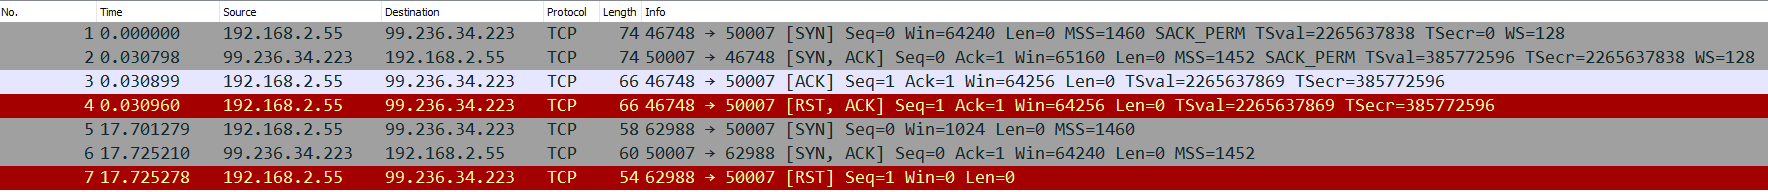
\includegraphics[width=\textwidth]{tcpdump_50007.png}
\end{figure}


\subsection*{TCP Scans of Closed Port 50009}
The filtered ports were assumed to be closed, and the scans were performed on the port 50009. A standard TCP connection scan (using -sT option) and a TCP SYN scan (using -sS option) of the server \texttt{compeng4dn4.mooo.com} on the closed port 50009 are performed and shown in Listing~\ref{list:nmap_50009}. For both scans, the Nmap scan reported the same information. The scans reported the same information on port 50009 as the earlier scans on the larger port range.

\begin{lstlisting}[caption=Nmap Scans on Port 50009,label=list:nmap_50009]
sudo nmap compeng4dn4.mooo.com -Pn -sT -p 50009
Starting Nmap 7.80 ( https://nmap.org ) at 2023-02-12 21:31 EST
Nmap scan report for compeng4dn4.mooo.com (99.236.34.223)
Host is up.
rDNS record for 99.236.34.223: cpe382c4a5bff48-cm00fc8db8cbb0.cpe.net.cable.rogers.com

PORT      STATE    SERVICE
50009/tcp filtered unknown

Nmap done: 1 IP address (1 host up) scanned in 2.12 seconds

sudo nmap compeng4dn4.mooo.com -Pn -sS -p 50009
Starting Nmap 7.80 ( https://nmap.org ) at 2023-02-12 21:32 EST
Nmap scan report for compeng4dn4.mooo.com (99.236.34.223)
Host is up.
rDNS record for 99.236.34.223: cpe382c4a5bff48-cm00fc8db8cbb0.cpe.net.cable.rogers.com

PORT      STATE    SERVICE
50009/tcp filtered unknown

Nmap done: 1 IP address (1 host up) scanned in 2.18 seconds
\end{lstlisting}

Both scans were captured with tcpdump, writing the scan to a WireShark compatible pcap file for analysis. The tcpdump packet capture command of the scans is shown in Listing~\ref{list:tcpdump_50009}. 

\begin{lstlisting}[caption=Tcpdump Packet Capture of Scans on Port 50009,label=list:tcpdump_50009]
sudo tcpdump -nnvvX -i 1 -S host compeng4dn4.mooo.com -w 50009.pcap
tcpdump: listening on eth0, link-type EN10MB (Ethernet), snapshot length 262144 bytes
4 packets captured
10 packets received by filter
0 packets dropped by kernel
\end{lstlisting}

The capture displayed in WireShark is shown below in Figure~\ref{fig:wireshark_50009}. The first two packets (1-2) are from the standard TCP connection scan on port 50009. The last two packets (3-4) are from the TCP SYN scan on port 50009.

The first two packets and last two packets both show the \href{https://nmap.org/book/synscan.html#scan-methods-fig-syn-scan-filtered}{expected behaviour of a Nmap scan on a filtered port}. The host (192.168.2.55) sends a SYN signal to the destination (port 50009 on 99.236.34.223) but does not receive a reply. After waiting some time (around 1 second in this capture), the host sends another SYN signal to try again. If the timeout period is again exceeded, Nmap will give up and mark the port as filtered.

\begin{figure}[htp]
\centering
\caption[tcpdump_50009]{Tcpdump Capture of Port 50009 in WireShark}\label{fig:wireshark_50009}
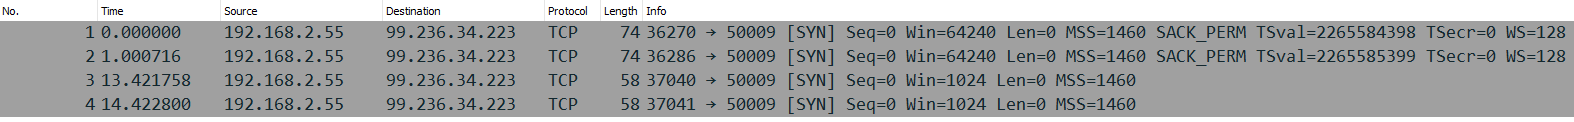
\includegraphics[width=\textwidth]{tcpdump_50009.png}
\end{figure}

\subsection*{Standard TCP Connection Scan of \texttt{localhost}}
A standard TCP connection scan (using -sT option) of \texttt{localhost} was performed and shown in Listing~\ref{list:nmap_localhost}. The scan reports all found open ports, and also states that there are 993 tcp ports that were filtered due to no-response. The services corresponding to each open port is also listed. The purposes of each service on these open ports are discussed in Table~\ref{tab:services}.

\begin{lstlisting}[caption=Nmap Standard TCP Connection Scan of \texttt{localhost},label=list:nmap_localhost]
nmap localhost -Pn -sT
Starting Nmap 7.93 ( https://nmap.org ) at 2023-02-11 23:39 Eastern Standard Time
Nmap scan report for localhost (127.0.0.1)
Host is up (0.00015s latency).
Other addresses for localhost (not scanned): ::1
Not shown: 993 filtered tcp ports (no-response)
PORT     STATE SERVICE
135/tcp  open  msrpc
445/tcp  open  microsoft-ds
2179/tcp open  vmrdp
5357/tcp open  wsdapi
9010/tcp open  sdr
9080/tcp open  glrpc
9100/tcp open  jetdirect

Nmap done: 1 IP address (1 host up) scanned in 44.45 seconds
\end{lstlisting}

\begin{table}[htp]
\centering
\caption[localhost_services]{Services on Open Ports of \texttt{localhost}}\label{tab:services}
\begin{tabular}{|l|l|l|}
\hline
PORT     & SERVICE      & PURPOSE                                   \\ \hline
135/tcp  & msrpc        & Microsoft Remote Procedure Call           \\ \hline
445/tcp  & microsoft-ds & Server Message Block (SMB)                \\ \hline
2179/tcp & vmrdp        & Microsoft RDP for virtual machines        \\ \hline
5357/tcp & wsdapi       & Microsoft Network Discovery               \\ \hline
9010/tcp & sdr          & Secure Data Replicator Protocol           \\ \hline
9080/tcp & glrpc        & Groove Collaboration software GLRPC       \\ \hline
9100/tcp & jetdirect    & HP JetDirect (for HP LaserJet printers)   \\ \hline
\end{tabular}
\end{table}

\subsection*{TCP Scan of Port 8000 on \texttt{localhost}}
A standard TCP connection scan (using -sT option) of port 8000 on \texttt{localhost} was performed and shown in Listing~\ref{list:nmap_localhost_8000}. The scan reports that the port is filtered (likely due to no response as mentioned in the previous report). The service that typically corresponds to this port is \texttt{http-alt}, an alternative HTTP port.

\begin{lstlisting}[caption=Nmap Standard TCP Connection Scan of Port 8000 on \texttt{localhost},label=list:nmap_localhost_8000]
nmap localhost -Pn -sT -p 8000
Starting Nmap 7.93 ( https://nmap.org ) at 2023-02-11 23:43 Eastern Standard Time
Nmap scan report for localhost (127.0.0.1)
Host is up.
Other addresses for localhost (not scanned): ::1

PORT     STATE    SERVICE
8000/tcp filtered http-alt

Nmap done: 1 IP address (1 host up) scanned in 2.11 seconds
\end{lstlisting}

\subsection*{TCP Scan of Port 8000 on \texttt{localhost} with HTTP Server}
A standard TCP connection scan (using -sT option) of port 8000 on \texttt{localhost} was performed while the HTTP server was running, and the scan is shown in Listing~\ref{list:nmap_localhost_8000_server}. The scan reports that the port is now open. When the web service is accessed through a browser, a page that serves the contents of the directory where the server was launched is shown. The webpage is shown in Figure~\ref{fig:server}.

\begin{lstlisting}[caption=Nmap Standard TCP Connection Scan of Port 8000 on \texttt{localhost} with HTTP Server,label=list:nmap_localhost_8000_server]
nmap localhost -Pn -sT -p 8000
Starting Nmap 7.93 ( https://nmap.org ) at 2023-02-11 23:43 Eastern Standard Time
Nmap scan report for localhost (127.0.0.1)
Host is up (0.0010s latency).
Other addresses for localhost (not scanned): ::1

PORT     STATE SERVICE
8000/tcp open  http-alt

Nmap done: 1 IP address (1 host up) scanned in 0.09 seconds
\end{lstlisting}

\begin{figure}[htp]
\centering
\caption[server]{\texttt{localhost:8000}}\label{fig:server}
\frame{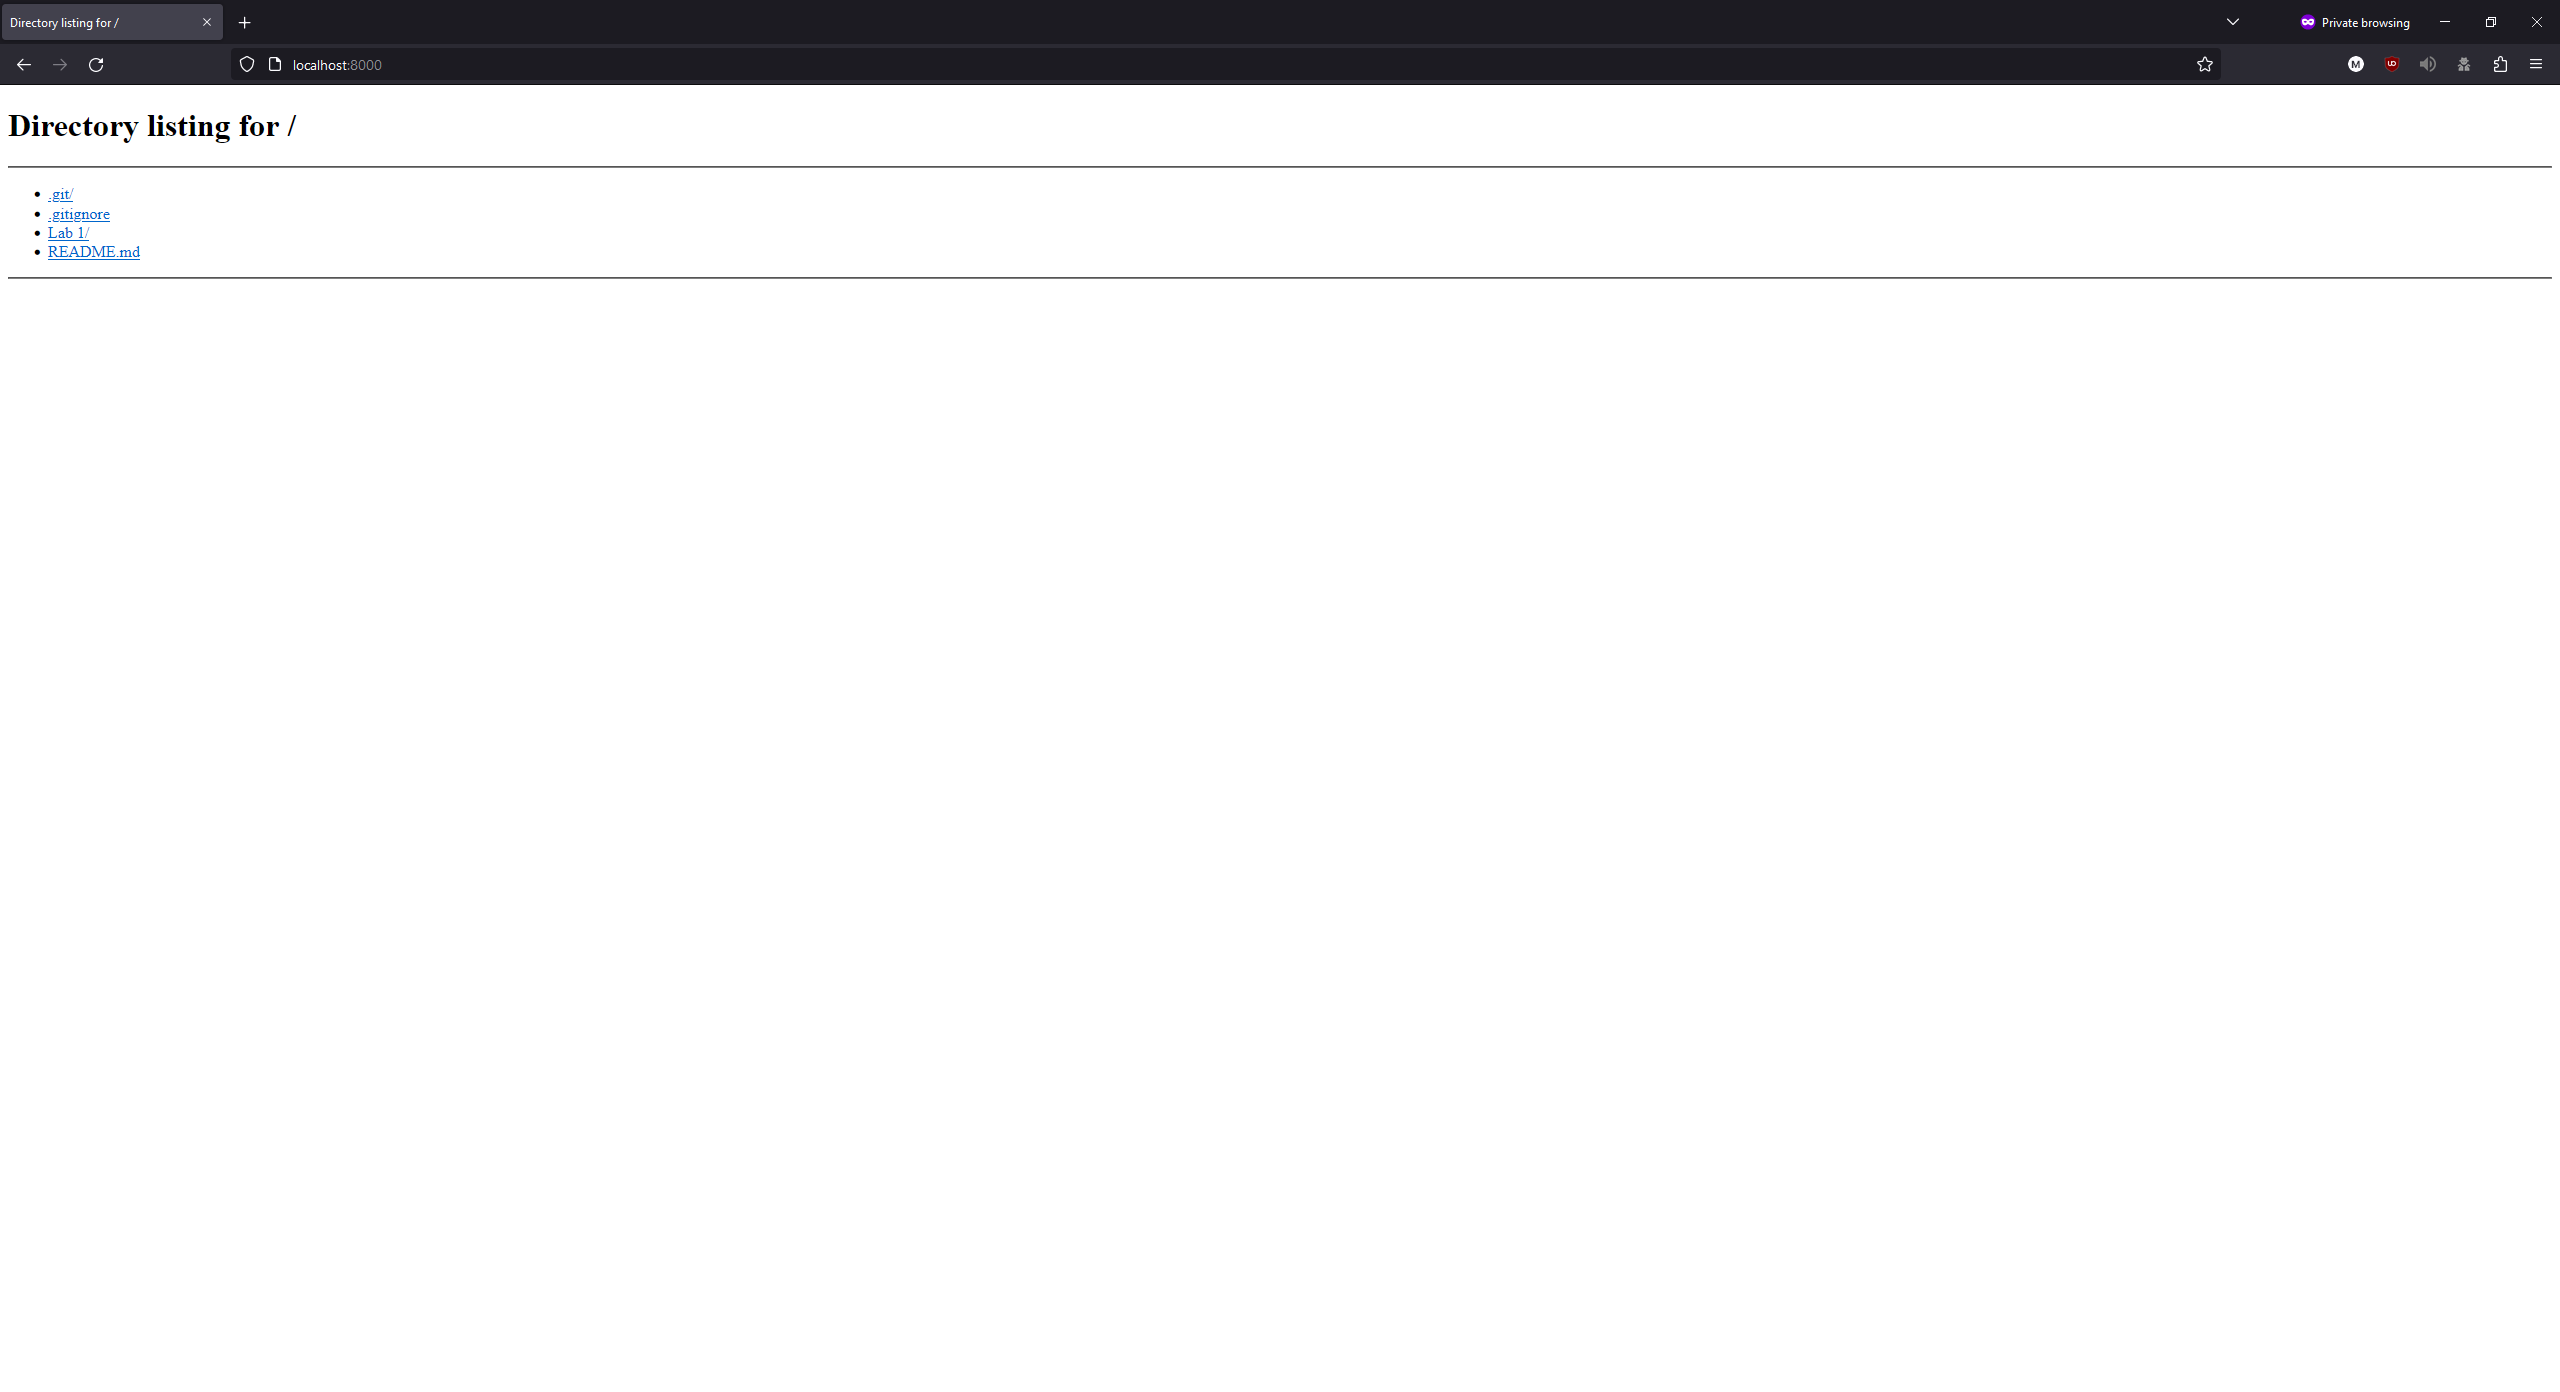
\includegraphics[width=\textwidth]{server.png}}
\end{figure}